% Regenerate with latex and dvisvgm; see graph-matching-common.tex.
% Shared styles for the vector replacements in graph-matching/.
% Compile each diagram from this directory, for example:
% latex -interaction=nonstopmode -halt-on-error augment-1.tex
% dvisvgm --no-fonts --exact --bbox=papersize -o augment-1.svg augment-1.dvi
\documentclass[tikz,border=5pt]{standalone}
\usepackage{lmodern,amssymb}
\usetikzlibrary{arrows.meta,backgrounds,calc}
\definecolor{matchred}{HTML}{D7191C}
\definecolor{matchblue}{HTML}{1748B5}
\definecolor{blossomgreen}{HTML}{087A16}
\definecolor{blossomfill}{HTML}{B3E3AF}
\tikzset{
  diagram/.style={x=1mm,y=-1mm,font=\small,line width=.6pt,
    line cap=round,line join=round,
    background rectangle/.style={fill=white},show background rectangle},
  vertex/.style={circle,draw,fill=white,minimum size=5mm,inner sep=0pt},
  point/.style={circle,fill=black,minimum size=2.8mm,inner sep=0pt},
  exposed/.style={point,draw=matchred,fill=matchred!80,line width=1pt},
  matching/.style={line width=2pt},
  transition/.style={-{Stealth[length=4mm,width=3mm]},
    line width=1.4pt,draw=matchblue},
  blossom/.style={draw=blossomgreen,fill=blossomfill,line width=1pt},
  route/.style={draw=matchred,line width=.9pt},
  label/.style={inner sep=1.5pt,align=center},
}

% The five-cycle has exactly two matching edges. Its exposed base is b0.
% Call inside a scope to translate the entire blossom consistently.
\newcommand{\FiveBlossom}{%
  \draw[blossom] (16,0) circle[radius=22mm];
  \foreach \id/\px/\py in {b0/0/0,b1/12/-16,b2/29/-9,b3/29/10,b4/11/16}
    \node[point] (\id) at (\px,\py) {};
  \draw (b0) -- (b1) (b2) -- (b3) (b4) -- (b0);
  \draw[matching] (b1) -- (b2) (b3) -- (b4);
  \node[label,text=blossomgreen,above] at (16,-22) {blossom};
  \node[label,text=blossomgreen,above=.3mm,xshift=-2mm] at (b0.north) {root};
  \node[label,below=.5mm] at (b0.south) {$v$};
}

\begin{document}
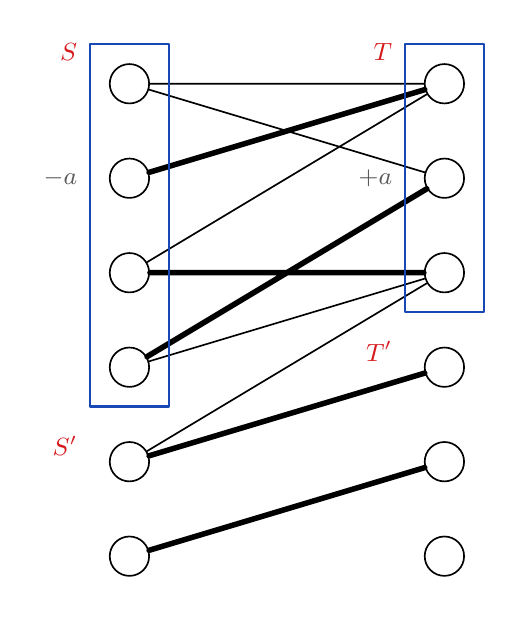
\begin{tikzpicture}[diagram]
  % S and T are the two sides of the alternating tree. The remaining
  % vertices form S' and T'. Thick edges are the current matching.
  \foreach \i in {1,...,6} {
    \node[vertex] (l\i) at (0,12*\i) {};
    \node[vertex] (r\i) at (40,12*\i) {};
  }
  \draw (l1) -- (r1) (l1) -- (r2) (l3) -- (r1)
    (l4) -- (r3) (l5) -- (r3);
  \draw[matching] (l2) -- (r1) (l3) -- (r3) (l4) -- (r2)
    (l5) -- (r4) (l6) -- (r5);
  \draw[matchblue,line width=.8pt] (-5,7) rectangle (5,53);
  \draw[matchblue,line width=.8pt] (35,7) rectangle (45,41);
  \node[label,text=matchred,left] at (-6,8) {$S$};
  \node[label,text=matchred,left] at (34,8) {$T$};
  \node[label,text=matchred,left] at (-6,58) {$S'$};
  \node[label,text=matchred,left] at (34,46) {$T'$};
  \node[label,text=black!65,left] at (-6,24) {$-a$};
  \node[label,text=black!65,left] at (34,24) {$+a$};
\end{tikzpicture}
\end{document}
